%!TEX root = knowledge-curation.tex
\section{Findings}
\label{cha:findings}

This section presents the findings of our study that answer each research question.
%	(1) a characterization of the non-mutually exclusive categories and properties of Stack Overflow and R-help mailing list according types of knowledge the channels contains;
%	(2) remarks about the ways knowledge is constructed on these two media channels;
%	(3) an explanation of how links support the construction of knowledge;
%	(4) a characterization of the knowledge based on the analysis of active users using both channels; and
%	(5) interesting remarks about users regarding their behaviour on these two media channels.

\subsection{RQ-1. What types of knowledge are shared on Stack Overflow and the R-help mailing list within the R community?}
%\section{Types of Knowledge}
\label{cha:findings-types}

	As mentioned above, the R-help is not a specialized mailing list, therefore we were motivated to investigate whether Stack Overflow shares the same types of knowledge as R-help.
	As a result, we identified five main types of knowledge from the messages from the Stack Overflow R tag and R-help mailing list:
	\begin{enumerate*}[label=(\arabic*)]
        \item Questions,
        \item Answers,
        \item Updates,
        \item Flags, and
        \item Comments.
	\end{enumerate*}
Each of them, with their sub-types of knowledge presented in Table~\ref{table:type-of-knowledge}.
Below we explain the five main type of knowledge, similarities and differences when they correspond.

\begin{table*}[!htb]
  \centering
  \caption{Types of knowledge found in both Stack Overflow and R-help.}
  \begin{small}
    \begin{tabularx}{\textwidth}{lX}
        \toprule
\multicolumn{2}{@{}l}{\textbf{Questions}}\\[0.2em]
    \emph{How-to} & Questions that ask how to do something specific.\\
	\emph{Bug/Error/Exception} & Questions that ask for a solution or reasons for a error message.\\
	\emph{Discrepancy} & Questions that ask about an unexpected result of a specific function, process, or package.\\
	\emph{Set-up} & Questions that ask for possible ways to set up the R environment before or after deployment.\\
	\emph{Decision help} & Questions that ask for advice in making a decision.\\
	\emph{Conceptual/Guidance} & The user requests a conceptual clarification or guidance on topics related with R or statistics.\\
	\emph{Code reviewing} & Questions that ask for code review, explicitly or implicitly.\\
	\emph{Non-functional} & Questions that ask for help (or suggestions) with a non-functional requirement such as performance, and memory usage.\\
	\emph{Future reference} & Questions a user ask---and normally answer itself---that might not exist on the channel, but that are interesting enough to create a thread for future reference.\\
	\emph{Other} & Questions that ask for assistance unrelated to the channel or the message contains unrelated information (e.g., announcements, ideas for improvement).\\[.4em]

\multicolumn{2}{@{}l}{\textbf{Answers}} \\[0.2em]
	\emph{Redirecting} & The user provides a link to an existing solution that is not in the thread (e.g. external application, tutorial, or project).\\
	\emph{Tutorial} & The user answers the question with a set of steps in order to teach people how to solve the issue.\\
	\emph{Source code} & The user provides a source code snippet as the solution without an extensive explanation about the answer.\\
	\emph{Clue/Suggestion/Hint} & The user provides possible ways to solve the issue without solving it.\\
	\emph{Alternative} & The user provides a different approach to a solution that is related to but not exactly what is being asked for (e.g. mathematical approach, data structure modification).\\
	\emph{Explanation} & The user explains an approach that answers the question and lists steps on how to do it.\\
	\emph{Announcement} & The user provides a notification about some artifact (e.g., packages, libraries).\\
	\emph{Benchmark} & The user provides a benchmark of multiple solutions posted by others or compares answers on the thread.\\
	\emph{Opinion} & The user provides their own opinion or expands other answers by adding scenarios and examples.\\[.4em]

\multicolumn{2}{@{}l}{\textbf{Updates}} \\[0.2em]
	\emph{Announcement} & Announces specific events (e.g., bounties, future updates).\\
	\emph{Background} & Adds additional context to the question or answer (e.g., what the user did previously or already knows).\\
	\emph{Correction} & Corrects format, grammar, spelling, and semantic mistakes.\\
	\emph{Expansion} & Expands the question or answer by providing scenarios or examples.\\
	\emph{Explanation} & Explains or clarifies a specific point in the question or answer, such as why the user chose a specific data structure, or the meaning of a variable.\\
	\emph{Solution} & The user answers their own question.\\[.4em]

\multicolumn{2}{@{}l}{\textbf{Flags}} \\[0.2em]
	\emph{Off-topic/opinion} & Identify questions that are unrelated to the list's interests or which answers are based on the opinion of channel participants (not actual facts). These flags can be assigned for different reasons or they can be used on different ways.\\
%	\begin{description}[itemsep=3pt, topsep=2pt, leftmargin=3em, parsep=0pt]
%		\item[\textit{Typographical error}:] A problem was caused by typographical error.
%		\item[\textit{Debugging help}:] User is asking help for debugging.
%		\item[\textit{Book, tool, software library}:] User is asking for a book, tool, software library, tutorial or other off-site resource.
%		\item[\textit{Minimal understanding}:] User did not demonstrate a minimal understanding of the problem being solved.
%		\item[\textit{Insufficient information}:] Question lacks sufficient information to diagnose the problem
%		\item[\textit{Extra information}:] User provide extra information that is unrelated to the question, but it might be of interest to whom asked the question.
%		\item[\textit{Homework}:] When users ask something that looks like an assignment.
%	\end{description}
	\emph{Not an answer}     & Emphasize \textit{alternative answers} out of the scope of the question, or to identify that a solution does not answer the question.\\
	\emph{Repeated question} & Acknowledge an user asking a repeated question.
	Either because the user could not find a proper answer that fits its needs or did not search the archives to see if the question was already asked.\\
	\emph{Too localized}     & Questions that are too specific and might not help any future reader.\\
	\emph{Unclear} & Questions that are difficult to understand.\\[.4em]

\multicolumn{2}{@{}l}{\textbf{Comments}} \\[0.2em]
	\emph{Clarification} & Provides (or requests) additional information about a question or answer.\\
	\emph{Expansion} & Provides additional information.\\
	\emph{Correction/alternative} & Suggests a change to a question or answer, offers an alternative solution or a correction.\\
	\emph{Compliment/criticism}   & Posts something good, offers thanks, provides an opinion or criticise someone.\\
	\emph{External reference}     & References an external resource.\\
        \bottomrule
    \end{tabularx}
  \end{small}
  \label{table:type-of-knowledge}
\end{table*}


\paragraph*{Questions and Answers}
These are similar in both channels. Questions express one or more problems or doubts faced by an user in Stack Overflow or R-help, whereas answers represent solutions to questions.
%We identified 10 type of knowledge related to \emph{questions}:
%	We identified 9 types of knowledge:

\paragraph*{Updates}
	A modification to a question or answer.
	On the R-help mailing list, updates are not easily identifiable as the communication is presented as plain text emails.
	Therefore, we defined updates on the R-help mailing list as \emph{emails submitted by the author of the question or answer}.

	In contrast, on Stack Overflow updates are presented in two ways:
	\begin{description}[itemsep=3pt, topsep=2pt, leftmargin=3em, parsep=0pt]
		\item[Labelled updates] are explicitly shown in the body of questions or answers next to a label that identifies the update (e.g., edit, update, and p.s.).
		When multiple update labels appear in a message, each label is accompanied by a number (e.g., \textit{``[Edit 1:]''} {\footnotesize URL:  \href{http://goo.gl/ptYAG0}{Q1452235}}), by a date (e.g., \textit{``Edit/Update (April 2011):''} {\footnotesize URL:  \href{http://goo.gl/ptYAG0}{Q1452235}}), or by a bulleted list (e.g., ``EDIT: - anova... -drop1...'' {\footnotesize URL:  \href{http://goo.gl/sQiq0M}{Q7273695}})

		\item[Non-labelled updates] are only visually recognizable through the message history system. The only indication of the change is a box at the end of the message that contains the user who performed the change and the date when it happened.
	\end{description}

	Depending of the type of update, the usage is different.
	Non-labelled updates are mainly used to correct format, grammar, spelling, and semantic mistakes, or to incorporate explanations, examples, and suggestions without changing the meaning of the question or answer. Labelled updates are for everything else.

%	We identified 6 types of knowledge related to \textit{updates}:

\paragraph*{Flags}

	On Stack Overflow, a flag is a mechanism to get a moderator's attention.
%	Flags are short announcements shown below a question, containing information about the alias of the user who flagged the question and the reason why it was flagged.
	Flags can accomplish different objectives: to mark messages as spam, rude or abusive behaviour; and, to identify duplicate questions, off-topic messages, unclear questions, opinion-based questions, and low-quality answers.
	Depending of the type of the flag, threads can be closed or users can lose reputation point.
%	Figure~\ref{fig:SOFlagsExample} depicts an example on a flagged message on Stack Overflow.

%	\begin{figure} [!htb]
%		\centering
%		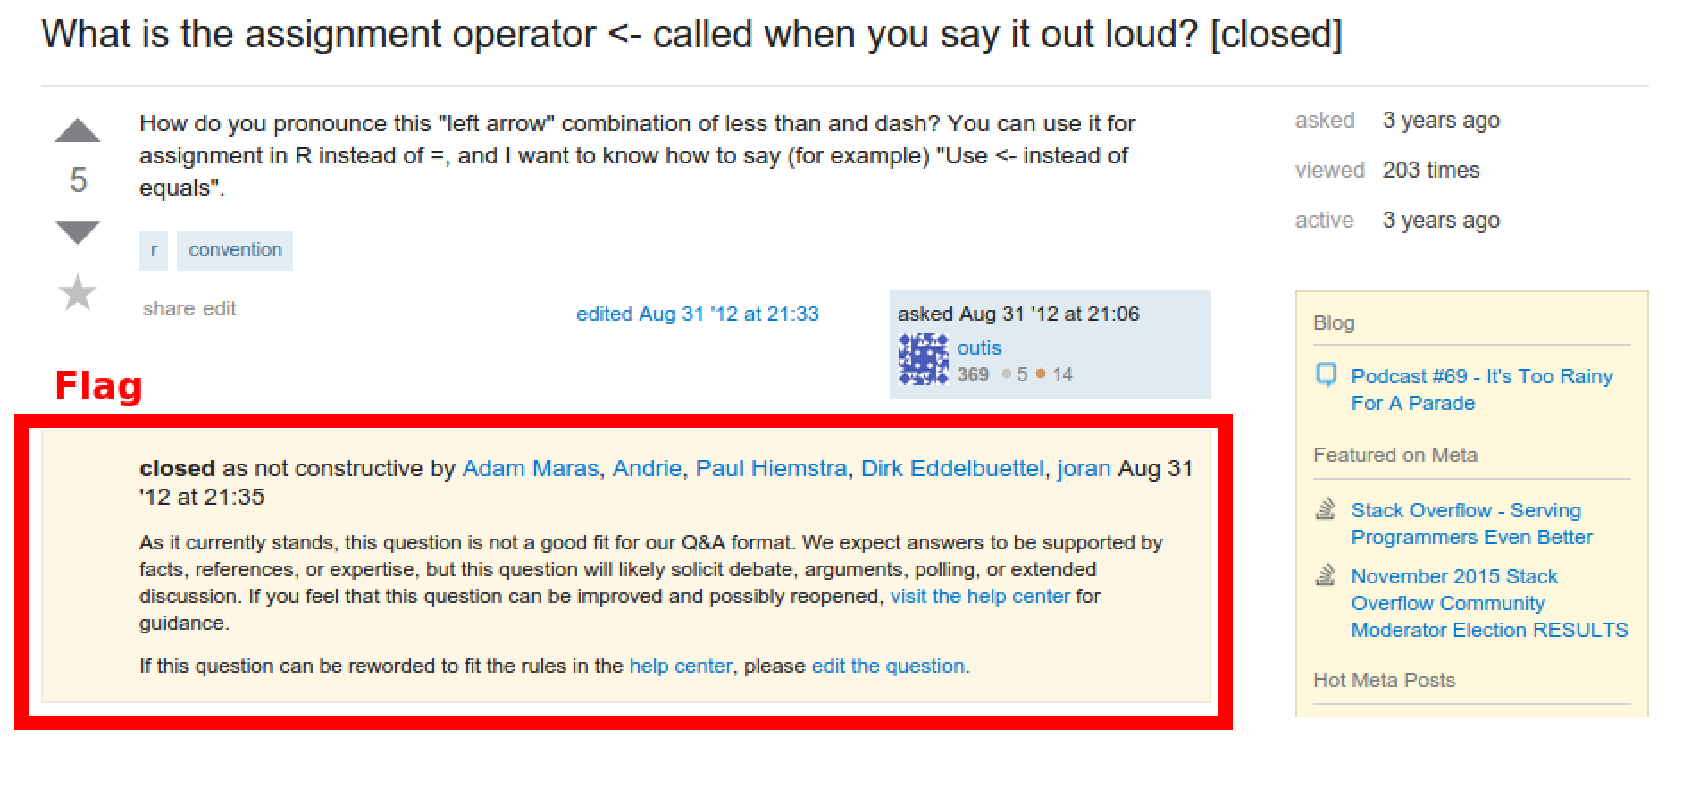
\includegraphics[width=\columnwidth]{Figures/SOFlagsExample}
%		\caption{Flagged post on Stack Overflow}
%		\label{fig:SOFlagsExample}
%	\end{figure}

On the R-help mailing list, the concept of flag does not exist. 
Based on the definition of flags on Stack Overflow, we defined flags as \emph{messages used to call the attention of other community members}.
Thus, flags on the R-help mailing list are used to keep a healthy community, promote discussion, and call the attention of community members to certain issues.
In contrast with Stack Overflow, flags might be used by the person who asked or answered a question.
Due to the format of messages on the R-help mailing list, flags can be mixed among the text of answers, comments, questions and updates.
	Flags in the R-help mailing list do not constrain users to answer questions, or to clarify what it is already asked.

%	We identified 6 types of knowledge related to \textit{flags}:

\paragraph*{Comments}
In Stack Overflow, comments are \textit{``temporary `Post-It' notes left on a question or answer..''}\footnote{\url{http://stackoverflow.com/help/privileges/comment}}.
	Comments are located below each question or answer, and can be used as a follow-up to questions, to answer a question, or to clarify a question.

	On the R-help mailing list, we defined comments as messages written to \emph{improve an answer in response to an incomplete question, or as a follow-up on a discussion}.
	Most importantly, messages should be written by a \emph{different person than the author of the question or answer} to which they are responding.
	In this context, the difference between an update and a comment is the motivation of the user who wrote the message and the author of the message.
%	For example, if user A posts a question, B asks A to clarify something about the question, and A answers back to B, then the last message is an update and the message sent by B to A is a comment (see Figure~\ref{fig:ExCommentUpdate1-1}).
%	Similarly, if user A posts a question, B answers A's question, A asks B to clarify something about the answer, and B answers back to A, then the second message is an answer, the third message is a comment, and the last message is an update (see Figure~\ref{fig:ExCommentUpdate1-2}).
%	% END>>

%	\begin{figure}
%		\centering
%	    \begin{subfigure}[b]{0.86\columnwidth}
%	      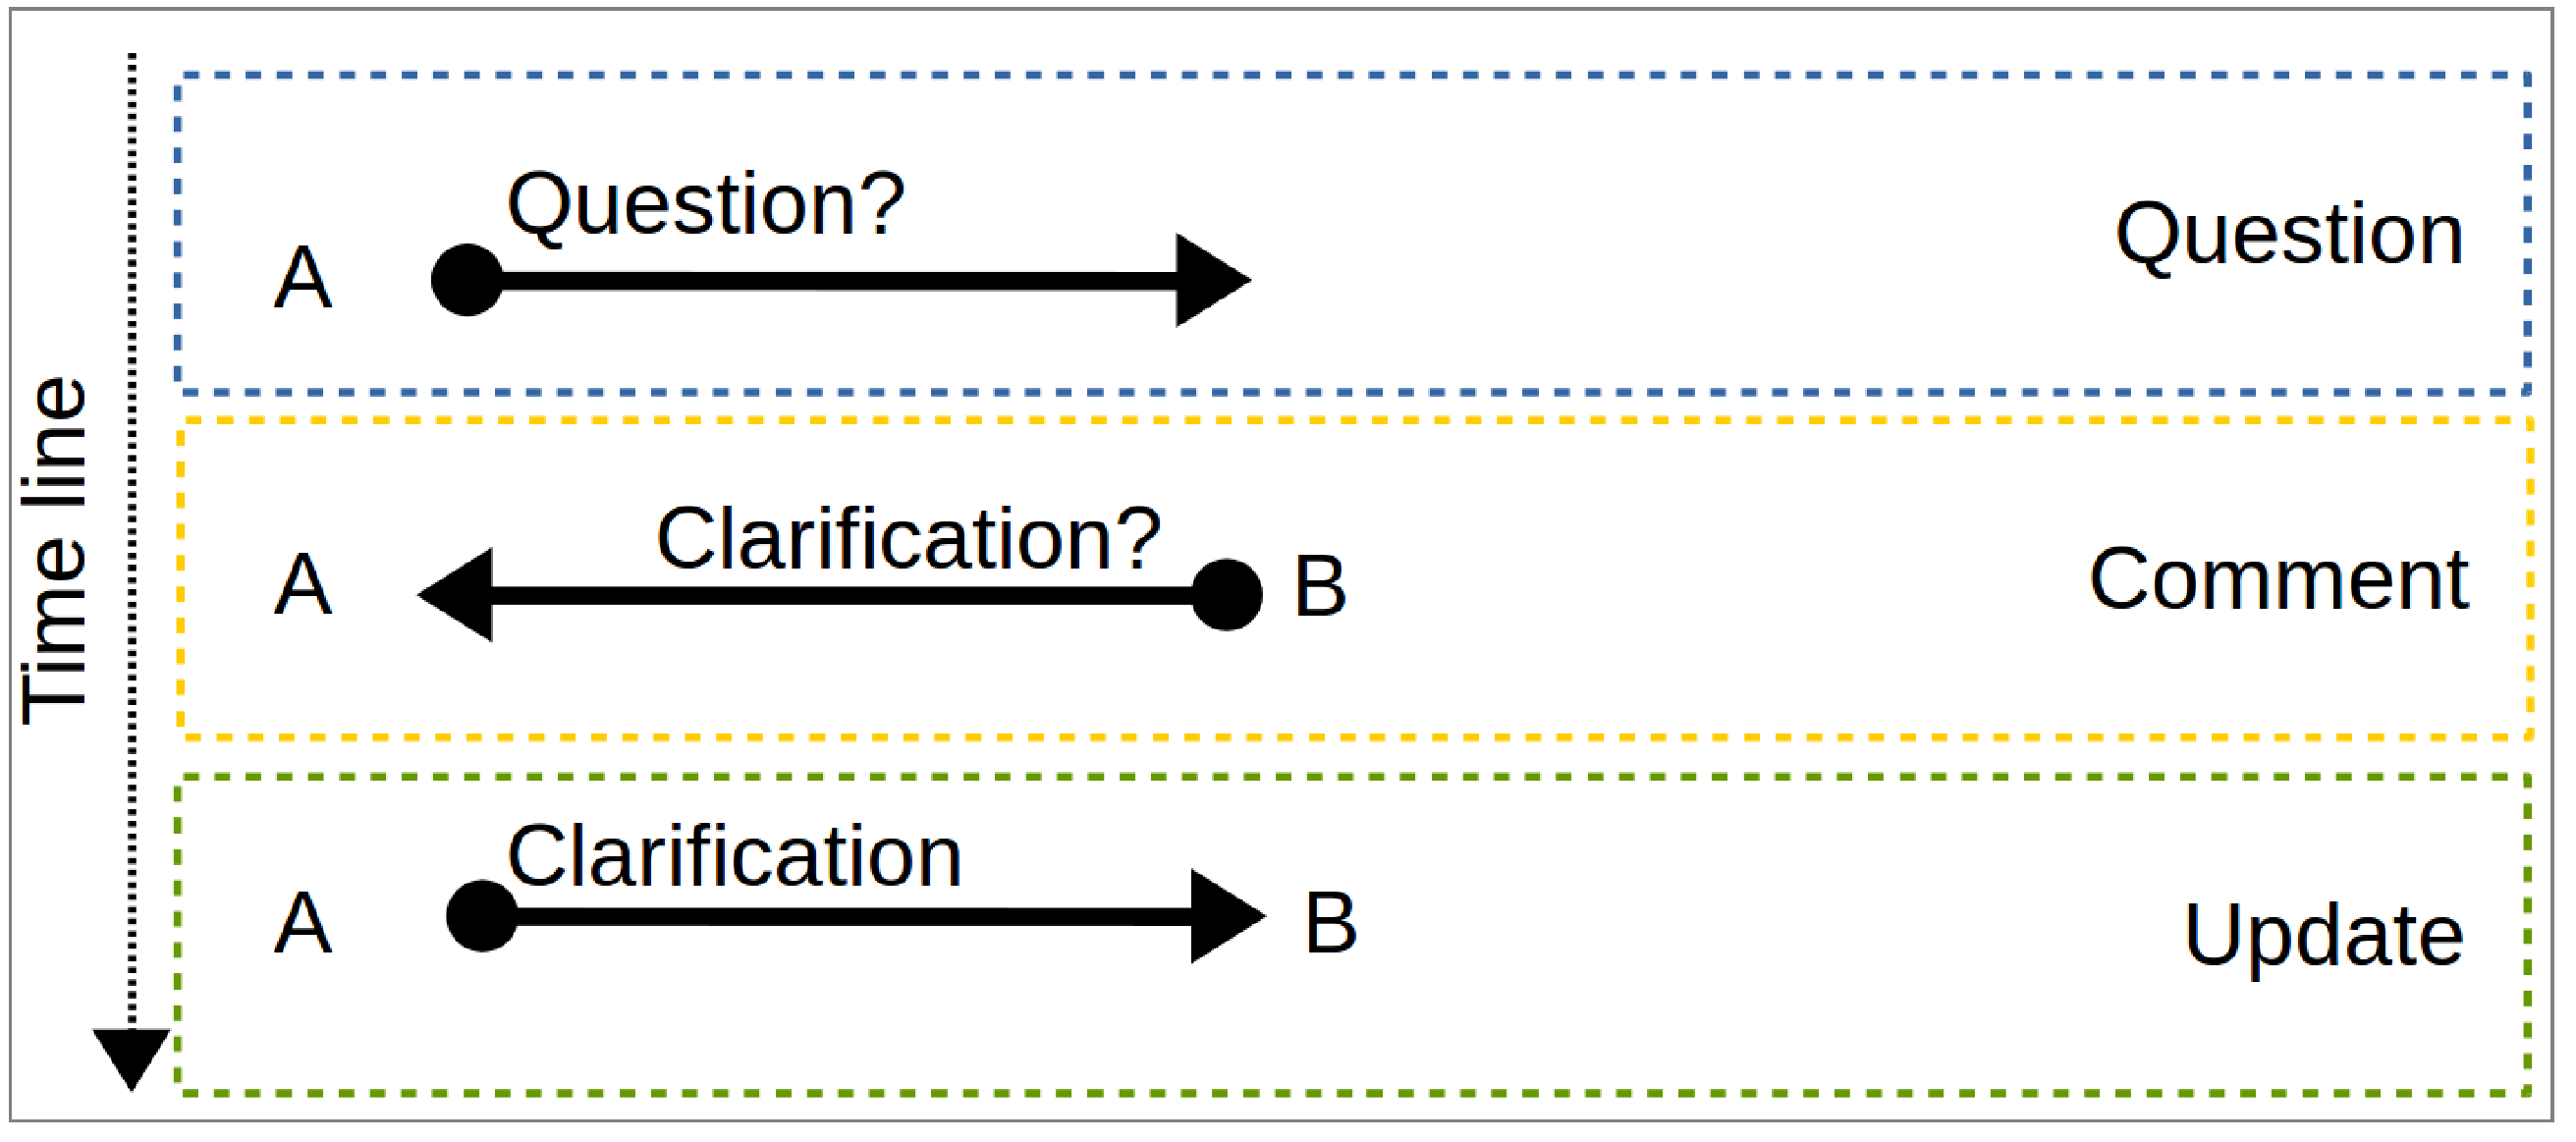
\includegraphics[width=\columnwidth]{Figures/ExCommentUpdate1}
%          \caption{A posts a question; later, B asks to A to clarify something about the question; and A answers back to B.}
%	      \label{fig:ExCommentUpdate1-1}
%        \end{subfigure}
%	    \begin{subfigure}[b]{0.86\columnwidth}
%	      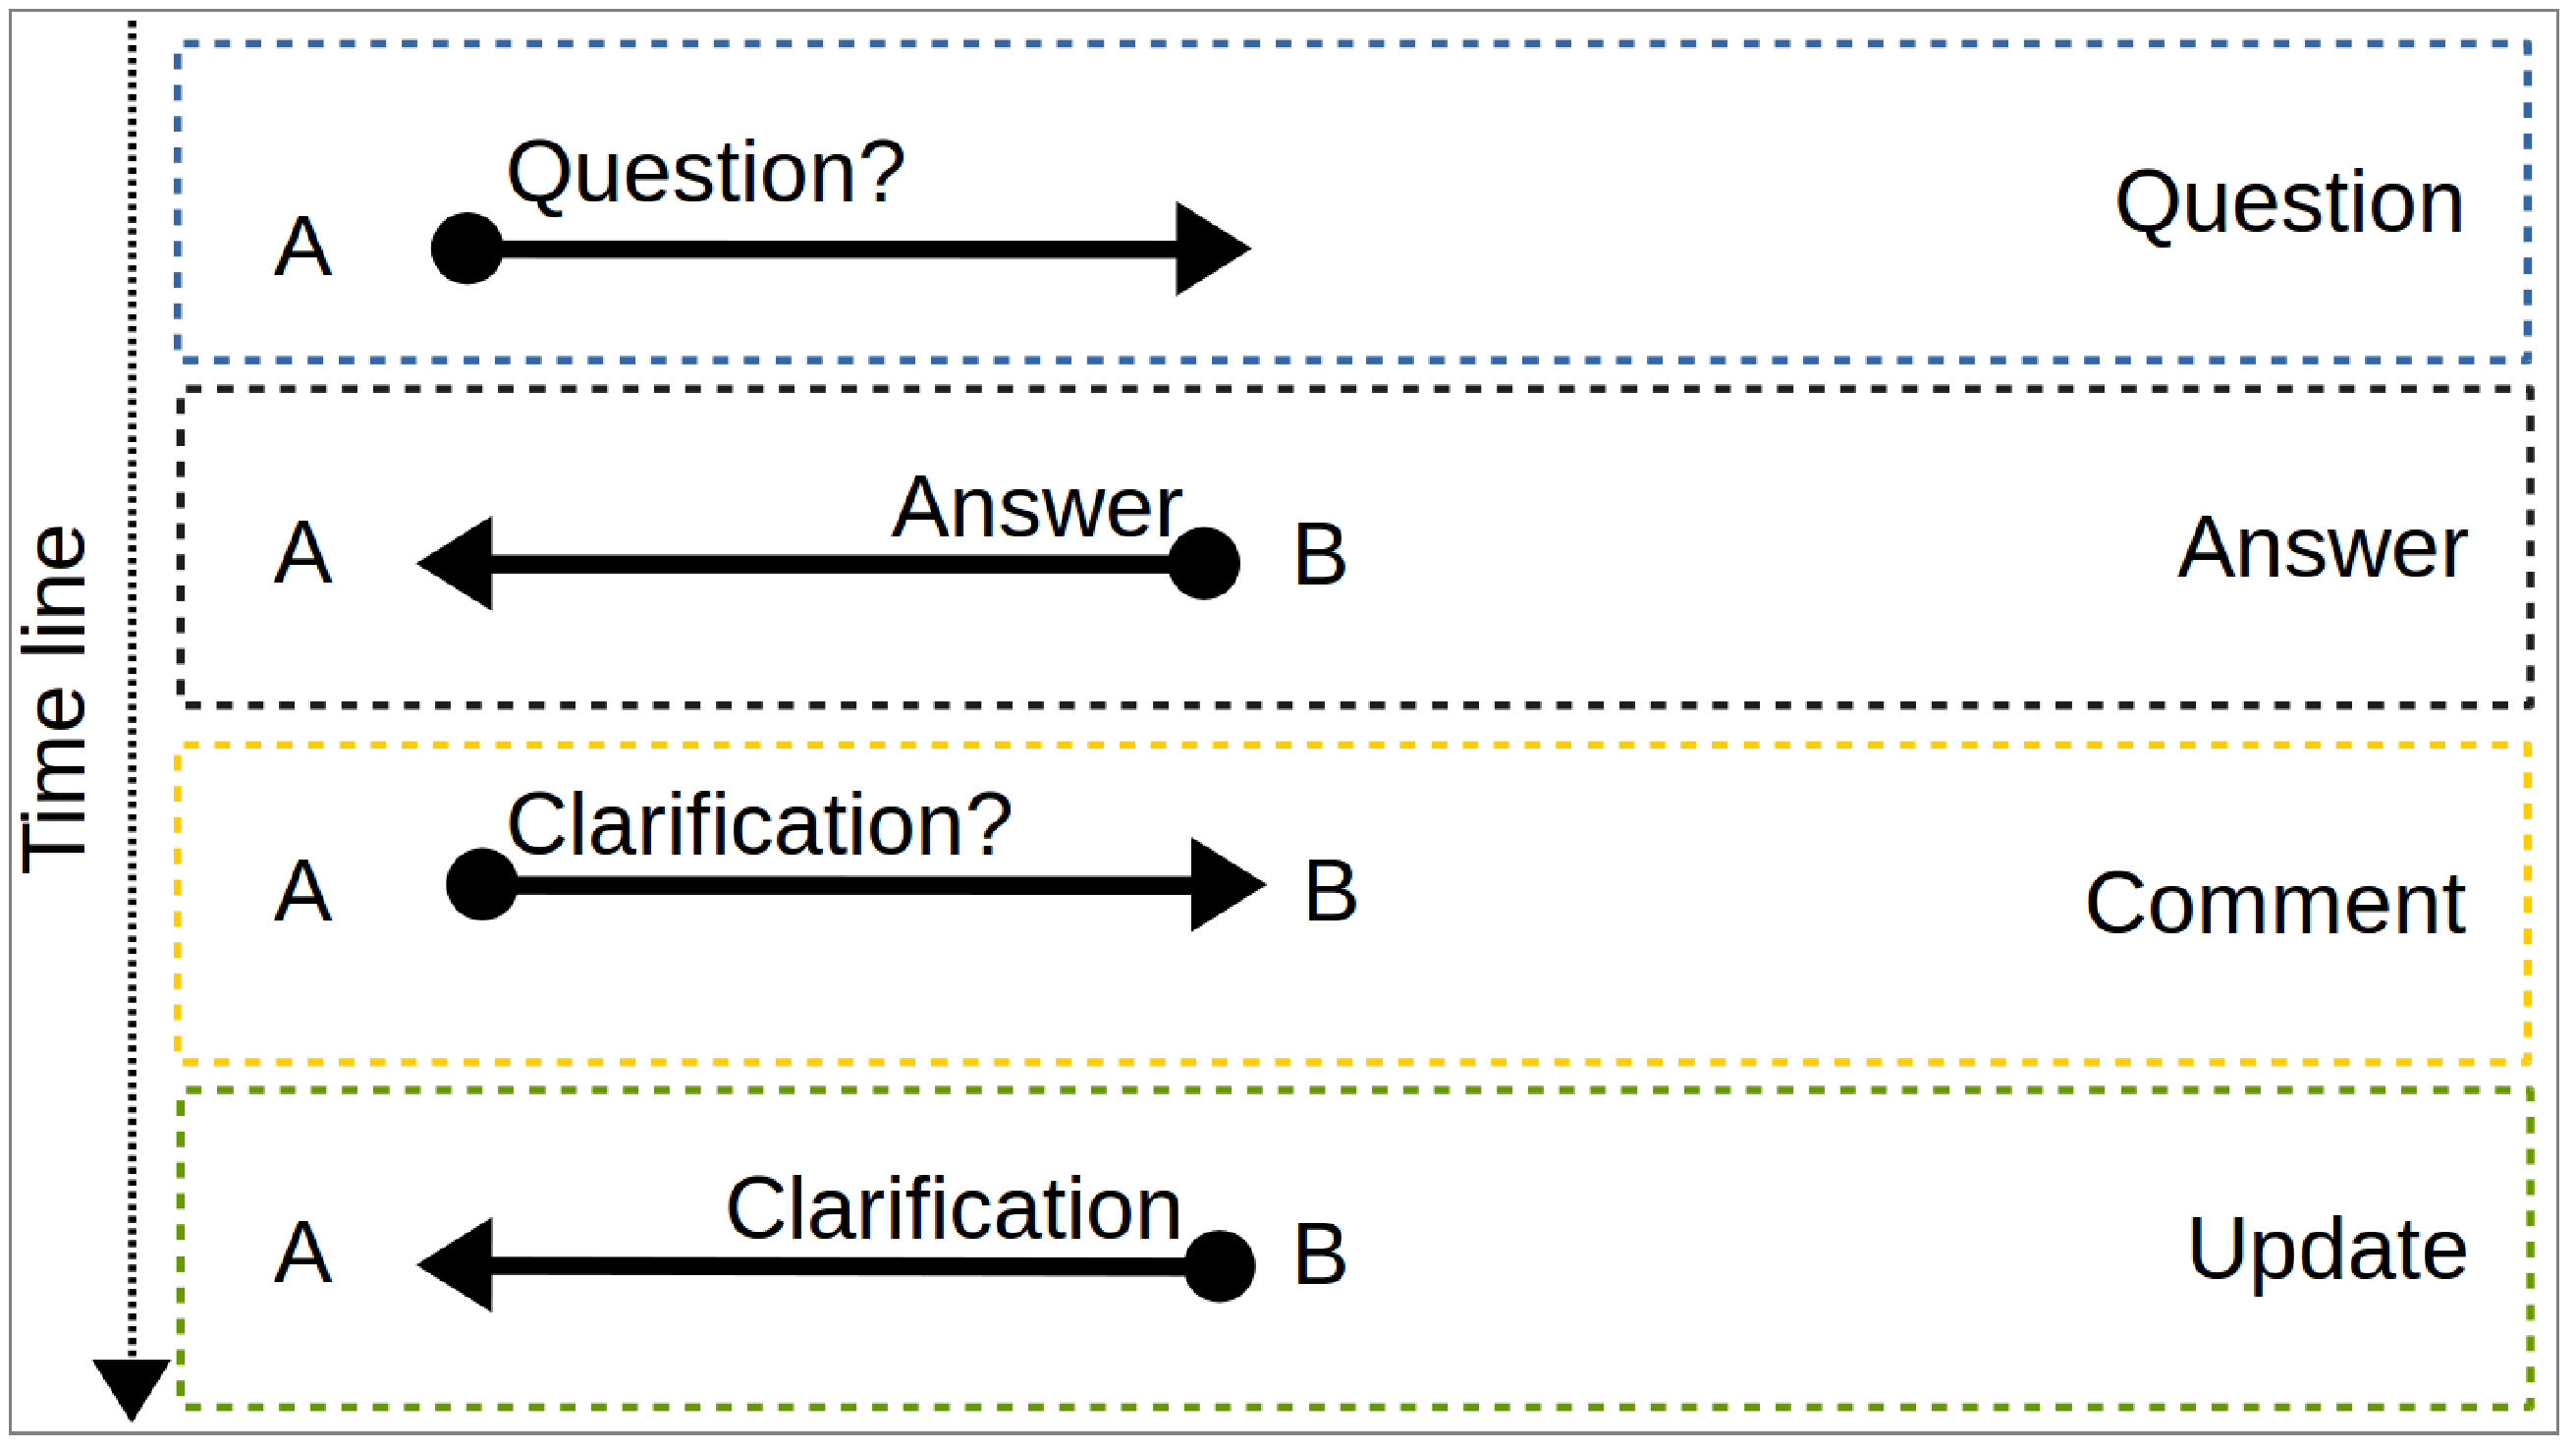
\includegraphics[width=\columnwidth]{Figures/ExCommentUpdate2}
%          \caption{A posts a question; later, B answers A's question; A asks to B to clarify something about the answer; and B answers back to A.}
%      	  \label{fig:ExCommentUpdate1-2}
%        \end{subfigure}

%		\caption{Two different interations. The arrows represent a message sent to the mailing list, and the labels specify the motivation behind the message.}
%		\label{fig:ExCommentUpdate1}
%	\end{figure}

%	We identified 5 types of knowledge related to \textit{comments}:

	The format of the message in Stack Overflow and the R-help mailing list, permits participants to ask multiple questions in the same thread.
	Therefore, the categorizations of knowledge presented in this section are non-mutually exclusive.

\subsection{RQ-2. How is knowledge constructed on Stack Overflow and the R-help mailing list?}
\label{sec:rq2}
%\section{Construction of Knowledge}

    %[Chapter Methodology]  We wondered if this applied to the creation and sharing of knowledge in these two channels. Our goal was to identify the mechanisms and strategies on Stack Overflow and the R-help mailing list used to construct knowledge collaboratively and individually (if any).

    Through our analysis, we identified two different approaches for constructing knowledge:
    \begin{packed_enum}
        \item \textbf{Participatory knowledge construction} are answers created through the cooperation of multiple users in the same thread.
        Participants complement each other's questions by providing pros and cons about the answer, different viewpoints, or additional context and examples.
        This is comparable with the concept of team in which people work together in a cooperative way for the same objective.

        \item \textbf{Crowd knowledge construction} leverages the experiences of many users; each user contributes its own explanations and practices adding variety to the pool of solutions.
        This is comparable with the concept of group in which people work towards the same objective but not necessarily together.
        Participants can vote over others ideas, but the idea is not constructed through a discussion process.
    \end{packed_enum}

    On the R-help mailing list, participatory knowledge takes place when:
    \begin{enumerate*}[label=(\arabic*)]
    \item previous answers are included in the actual answer and it is possible to infer a link between them; or
    \item when a in the message contains a direct reference to other answers or authors.
    \end{enumerate*}
    Figure \ref{fig:ML-PK1} depicts two examples of the way participatory knowledge occurs on the R-help mailing list:
    direct citation of the author of a previous answer (top), and inferable links between answers (right).

    
    \begin{figure}[!htb]
        \centering
        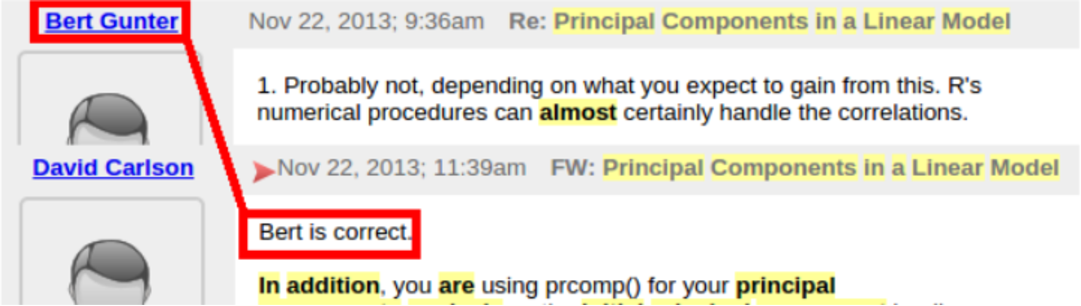
\includegraphics[width=.85\columnwidth]{Figures/ML-PKimg2}
        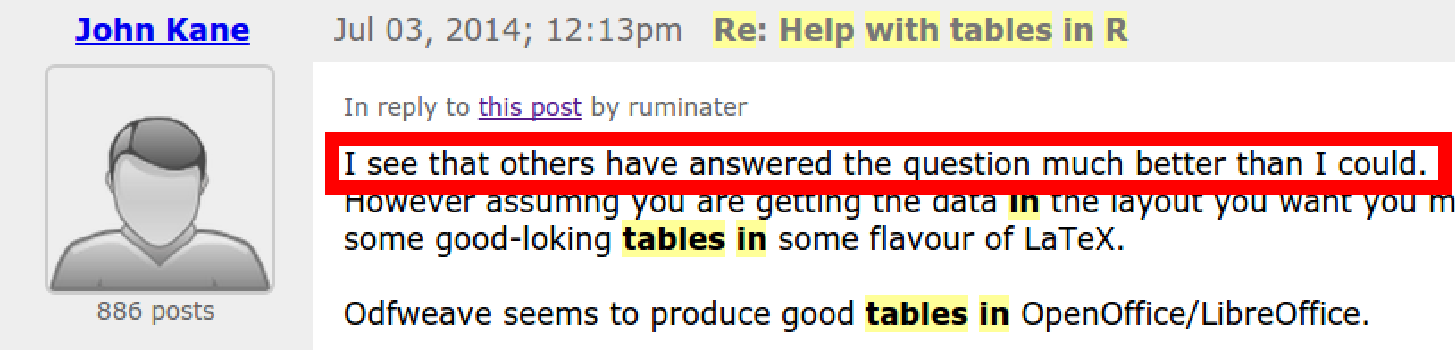
\includegraphics[width=.85\columnwidth]{Figures/ML-PKimg11}
        \caption[Participatory knowledge on the R-help mailing list.]{Participatory knowledge on the R-help mailing list.}
        \label{fig:ML-PK1}
    \end{figure}

    On Stack Overflow, participatory knowledge takes place when:
    \begin{enumerate*}[label=(\arabic*)]
    \item it is possible to infer a link between answers, via either a direct or indirect reference; or
    \item comments complement the answer, or directly cite another author.
    \end{enumerate*}

    On Stack Overflow, participatory knowledge happens in different places, perhaps as a consequence of its rich interface.
    We observe this phenomena, when a user answers a question and directly cites or links to the author of another answer in the thread, or when a user cites the author of a question or answer in a comment made on that question or answer, by including more information, or by suggesting that the answer provided is an additional solution.
    Figure \ref{fig:SO-PK1} depicts an example of participatory knowledge in Stack Overflow: the author participate in the comments to help another user when the answer is not sufficient for a particular case.
    In the comment, the user references another authors and answer.

    \begin{figure}[!htb]
        \centering
        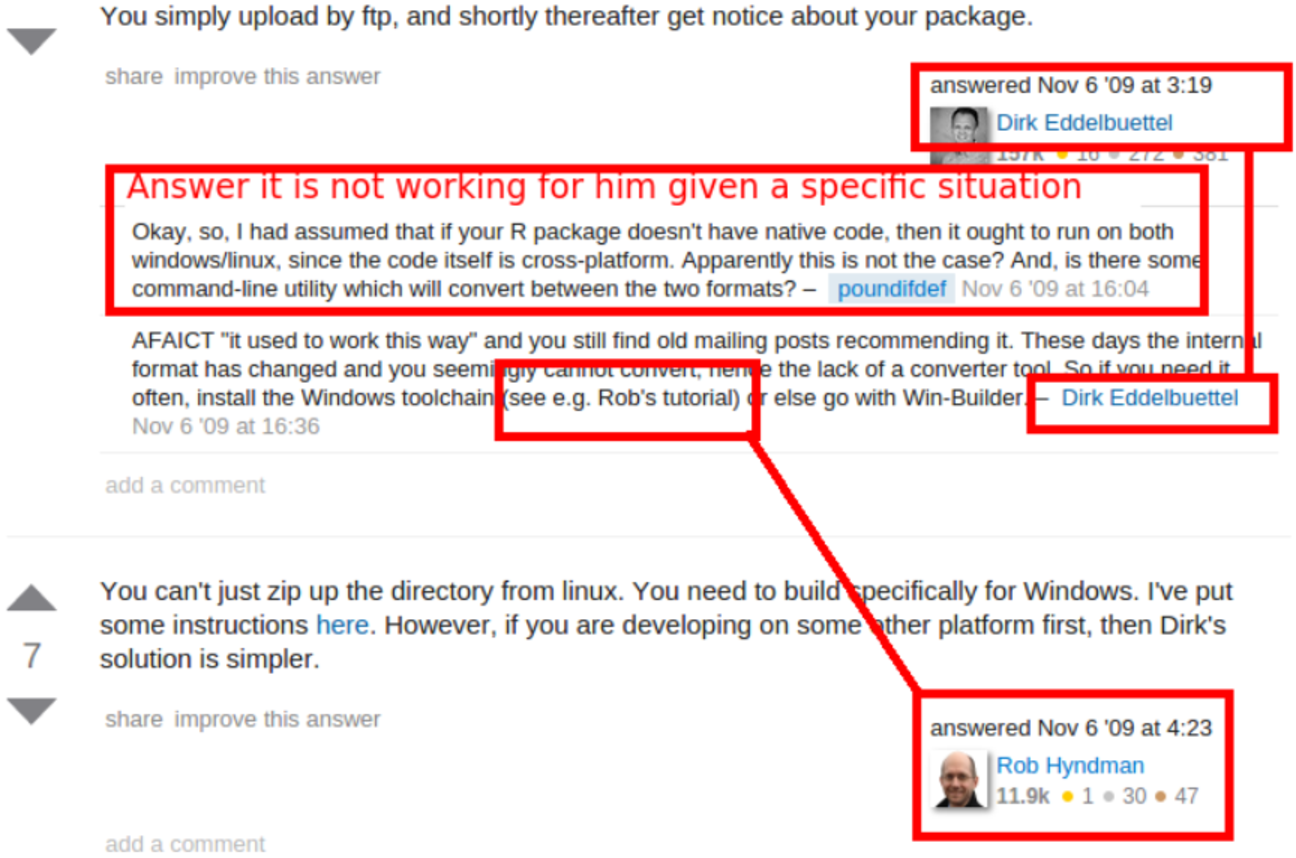
\includegraphics[width=.9\columnwidth]{Figures/SO-PKimg5}
        \caption{Example of participatory knowledge on Stack Overflow.}
        \label{fig:SO-PK1}
    \end{figure}

    Crowd knowledge construction is observable when:
    \begin{enumerate*}[label=(\arabic*)]
    \item there is not a direct or inferable reference between answers,
    \item answers are a variation of one of the answers on the thread.
    \end{enumerate*}
    Figure \ref{fig:CKC_MLSO} depicts an example of how crowd knowledge construction is visible on Stack Overflow.
    As can be seen from the figure, there are two of the three answers that provided a repeated solution.

%   \remarks{FIX THE FIGURE}

    \begin{figure} [!htb]
        \centering
        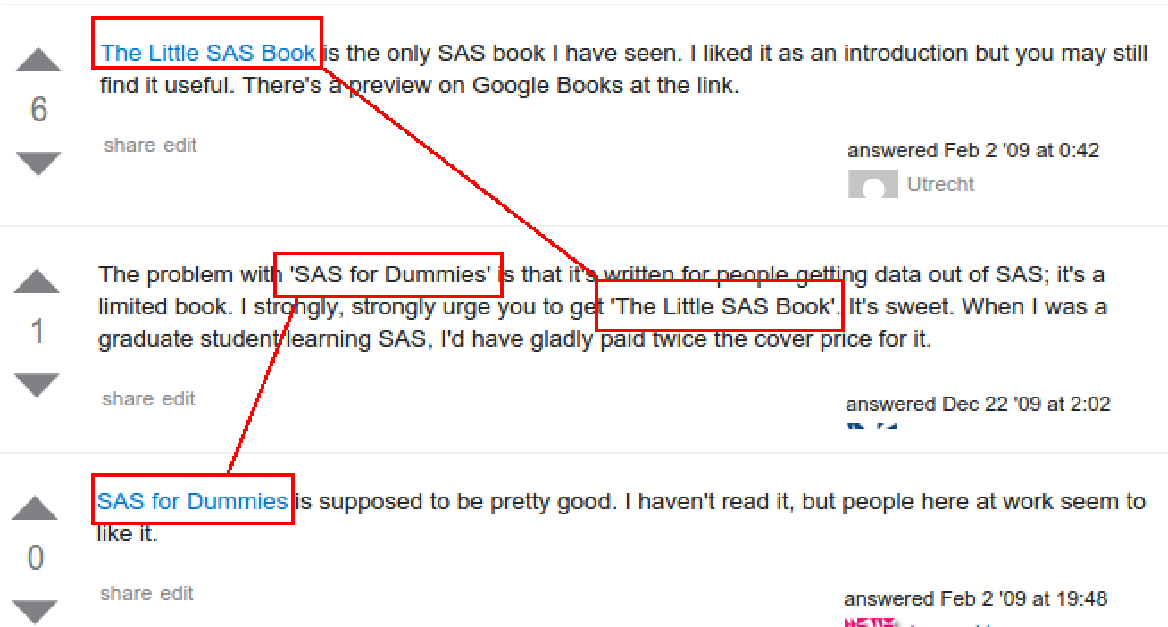
\includegraphics[width=.9\columnwidth]{Figures/SO-CSimg2}
        \caption{Example of how crowd knowledge construction occurs.}
        \label{fig:CKC_MLSO}
    \end{figure}

%\subsection{RQ-3. How does the sharing of links on Stack Overflow and the R-help mailing list support knowledge construction? }
%%\section{External Resources and the Construction of Knowledge}

%   % [Chapter Methodology] We wondered if this was also true for the R-help mailing list. More importantly, we wanted to know how this network of links contributes to the construction of knowledge.

%   External resources contain information that is valuable for questions and answers.
%   More importantly, they contribute to the construction of knowledge, often by simplifying answers and other contributions.
%   However, depending on the type of resource (e.g., forum, Q\&A Website, or Wiki), the support might be different.
%   % <<UPDATED 08-12-2015 BEGIN
%   We found that each type of resource is shared and supports knowledge on Stack Overflow and the R-help mailing list in the same way.
%   % END>>

%   Our analysis showed that there are 11 resource types:
%   \begin{packed_enum}
%       \item \textbf{Q\&A channels}: A online media channels for asking questions and answers (e.g., Stack Overflow and the R-help mailing list).
%       \item \textbf{Source code management systems, project hosting or issue trackers}: Online services that provided support for management of changes to documents (e.g., GitHub), hosting of projects (e.g., SourceForge or Google Code), and management of the software issues (e.g., Bugzilla).
%       \item \textbf{File hosting}: Online services that provide support for management of files (e.g., MediaFire and Dropbox).
%       \item \textbf{Digital Libraries, papers, books and journals}: Online services that provide access to papers, books, journals (e.g., R Journal arXiv).
%       \item \textbf{Forums}: Online discussion website where people can hold conversations in the form of posted messages (e.g., Google Groups).
%       \item \textbf{Wiki}: Online website that allows collaborative modification of its content through the web browser (e.g., Wikipedia).
%       \item \textbf{Blog}: An informal website to published discussion, ideas, and tutorial (e.g., Wordpress).
%       \item \textbf{Official documentation}: Documentation published by the original source of the technology (e.g., CRAN)
%       \item \textbf{Libraries, packages and applications}: collection of non-volatile source code or resources used by programs (e.g., GGPLOT) or entire software solutions (e.g., RSTudio)
%       \item \textbf{Online environments}: website that provide online environments such as IDE or notepads with source code syntax highlighting (e.g., GitHub Gits, or Pastebin)
%       \item \textbf{Other}: Websites from companies, non- official documentation sites, or any other online services do not include on the previous resources list.
%   \end{packed_enum}

%   Additionally, we identified 10 types of resources that are linked to support knowledge construction:
%   \begin{packed_enum}
%       \item \textbf{Answers}: Links to an answer on a Q\&A media channel.
%       \item \textbf{Tutorial/Guide}: Links to tutorial or guides.
%       \item \textbf{Source code/Examples}: Links to source code example, implementation, or final products.
%       \item \textbf{Channel}: Link to a an specific media channel.
%       \item \textbf{Expand/Background}: Links to a source of information that should be read.
%       \item \textbf{Books and papers}: Links to books, papers, and journals
%       \item \textbf{Hacks}: Links to workarounds.
%       \item \textbf{Images}: Links to images.
%       \item \textbf{Data}: Links to data.
%       \item \textbf{Announcement}: Links to company or personal webpage or project.
%   \end{packed_enum}

\subsection{RQ-3. Why do certain users post to both Stack Overflow and the R-help mailing list}
%\section{Characterization of the Knowledge \\from Active Users}

    For a community such as R, the variety of channels makes it possible to reach different users of the same community.
    Therefore, it is possible to find that a question is posted in both channels by the same user.
    We were motivated to understand the reasons, as well as the benefits or disadvantages of posting the same questions in both channels at the same time.

    We identified that being active on both channels at the same time brings some benefits:
    \begin{packed_enum}
        \item \textbf{Improve the existing answer:} If a question has no answer in one channel, an answer may exist in the other channel.
        \item \textbf{Support follow-up questions:} If a question is already closed and further questions arise, users can use other channels to reach out for help.
        \item \textbf{Speeds up answers:} Users can ask the same question on both channels to speed up the process, and at the same time, get more points of view. However, this behaviour is not encouraged by the community as it is deemed impolite.
    \end{packed_enum}

\subsection{User Behaviours}
\label{sec:userbeh}

    While analysing questions and answers, we identified user behaviours that are not reflected in the categories we developed, but that we believe are worth mentioning.
    These behaviours provide evidence of their altruistic way of thinking and the strong commitment that users have within the community.
    \begin{packed_enum}
        \item \textbf{I answered my own question}: Some questions are answered by the same user who asked the question. They posted back to the channel to document their solution.
        For example, \textit{\href{http://goo.gl/FG59Mw}{``I've discovered the answer to my own question.''}} or \textit{\href{https://goo.gl/r3z0DX}{``Just for the records (and if anyone ever wants to find the ``solution"), I solved my own problem.''}}.

        \item \textbf{I did it for you}: When answering authors provide an extensive amount of source code to help others. For instance, \textit{\href{http://goo.gl/GXWGG3}{``I have coded up the algorithm from the Cameron and Turner paper. Dunno if it gives exactly the same results as my (Splus?) code from lo these many years ago...''}}.

        \item \textbf{Answered, updated or continued years later}: Some answers are provided months or years after the question was asked.
        For instance, \href{http://goo.gl/k6ZARR}{a user on Stack Overflow modified an answer to provide a more updated version of the source code}; and a \href{http://goo.gl/kgSHZv}{question asked on the R-help mailing list in 2012 was continued two years later}.

        \item \textbf{Ideas for improvement or creation of the channel}: This behaviour is specific for the R-help mailing list. Sometimes users suggest modifications or new features to improve the channel. For instance, a \href{http://goo.gl/p0IunD}{user proposes to create a package repository that can be accessible through a public wiki, or version control interface}.
%       There are also messages to motivate community members to generate new ideas. For instance, a user encourages the community to provide new ideas to improve a well known site for review and tag R packages (i.e.,{\footnotesize \href{http://goo.gl/63AFxN}{Q63AFxN}}).
%       Finally, a user proposes to discuss the future of the R-help mailing list given the existence of Stack Overflow ({\footnotesize URL:  \href{http://goo.gl/GtUpfb}{QGtUpfb}}).
    \end{packed_enum}

    We also identified 2 behaviours that might result in a bad response from the community:
    \begin{packed_enum}
        \item \textbf{Cross-posting:} The user posts the same question in both channels at the same time.
        For instance: \textit{\href{http://goo.gl/ENKrVK}{``-1 for cross posting to r-help – [user name]''}}.
        \item \textbf{Posting guidelines violation:} The user behaves in a way that it becomes apparent that they did not read the posting guidelines.
        For instance, a user asked a question that seems to be the opposite of what the posting guide recommend, and someone answered: \textit{\href{http://goo.gl/FUm1HC}{``...If you read the Posting Guide I think you will find precisely the opposite expectation explicitly presented. Using my "cheeky code" would only be part of the recommended actions to take before posting if you follow the recommendations of the "Do your homework before posting:"...''}}.
    \end{packed_enum}

\subsection{Survey results}
\label{sec:survey}

The objective of the survey was to bring further insights on the study.
In the survey, the main findings came from the open questions that gather information about the experiences of the participants on Stack Overflow and the R-help mailing list.
Given the nature of this study, we were interested in the opinions regarding the preferences of one channel over the other, as well as any challenges that the participants might have experienced.
These questions were intended to provide insights to understand why these channels are used, as well as some opportunities for improvement.

%   {\itshape
%   \begin{itemize}
%       \item Have you experienced any challenges using Stack Overflow? Please elaborate.
%       \item What motivates you to answer questions or add comments on Stack Overflow? Please elaborate.
%       \item Have you experienced any challenges using the R-Help Mailing List? Please elaborate.
%       \item What motivates you to answer questions on the R-Help Mailing List? Please elaborate.
%       \item Why do you think the R-Help Mailing List has been replaced by Stack Overflow? Please elaborate.
%       \item In what situations would you choose Stack Overflow over the R-Help Mailing List? Please elaborate.
%       \item In what situations would you choose the R-Help Mailing List over Stack Overflow? Please elaborate.
%   \end{itemize}
%   }

    The reported benefits of using Stack Overflow were as follows: peer recognition, a friendly and rich interface, answers are straight to the point, it is easy to search for information, and questions are answered faster.
    However, the drawbacks of Stack Overflow include: strict rules become an obstacle sometimes and add complexity, the abundance of related questions, certain level of experience is required to understand the answers, and limitations on the scope of topics to discuss.

    The benefits of using the R-help list include: the convenience of just handling email, the information can be used to learn, the answers are more focused, the participation of highly experienced users (i.e., rock stars), and its flexibility.
    The disadvantages that were reported include: sometimes there can be aggressive behaviour, performing search is not easy, email is not a desirable interface, and the lack of categorization given the massive volume of information.

In the following sections we provide selected quotes from the survey.
Each participant is identified by an \emph{U} and a number (U\#).
